\documentclass[tikz,border=10pt]{standalone}
\usetikzlibrary{calc,intersections}

\begin{document}
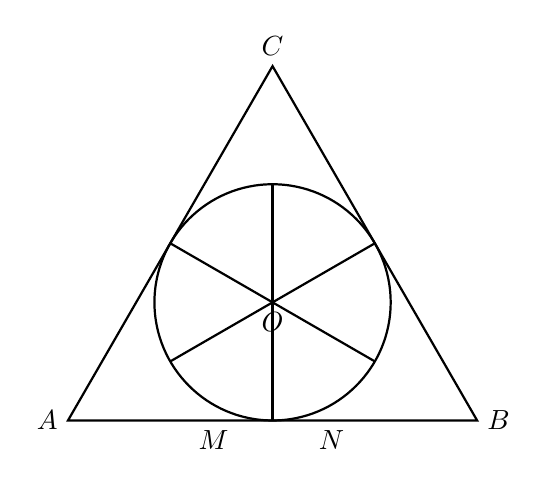
\begin{tikzpicture}[line width=0.8pt]

    % 定义基础参数
    \def\r{1.5} % 圆的半径
    \coordinate (O) at (0,0); % 圆心 O
    
    % 绘制圆
    \draw (O) circle (\r);
    
    % 定义三角形 ABC 的顶点
    % 基于边长关系，计算得到的高和底边位置
    \coordinate (A) at ({-2*\r*sin(60)},{-\r});
    \coordinate (B) at ({2*\r*sin(60)},{-\r});
    \coordinate (C) at (0,{2*\r});
    
    % 绘制三角形 ABC
    \draw (A) -- (B) -- (C) -- cycle;
    
    % 定义圆周上及边上的关键点
    \coordinate (M) at (-0.75, -\r);
    \coordinate (N) at (0.75, -\r);
    
    % 绘制内部连线 (分割线，以 O 为中心)
    \draw (O) -- ++(90:\r) coordinate (P1);
    \draw (O) -- ++(150:\r) coordinate (P2);
    \draw (O) -- ++(210:\r) coordinate (P3);
    \draw (O) -- ++(270:\r) coordinate (P4);
    \draw (O) -- ++(330:\r) coordinate (P5);
    \draw (O) -- ++(30:\r) coordinate (P6);
    
   
    % 标记点
    \node[below] at (O) {$O$};
    \node[left] at (A) {$A$};
    \node[right] at (B) {$B$};
    \node[above] at (C) {$C$};
    \node[below] at (M) {$M$};
    \node[below] at (N) {$N$};

\end{tikzpicture}
\end{document}